Luego del proceso de anotaci\'on y correcci\'on de lemas y etiquetas gramaticales,
se extrajeron algunas m\'etricas de resumen y se realizaron gr\'aficos con el fin de
comprender qu\'e distribuci\'on presentaban dichas etiquetas utilizadas y cu\'antos de los
datos etiquetdados de forma autom\'atica requirieron alguna correcci\'on, ya fuera en el
lema asignado, ya en la etiqueta gramatical predicha.
\par
En total, se revisaron 8324 anotaciones\footnote{Cada anotaci\'on est\'a dada por
la ocurrencia \textit{cruda} de la palabra, la etiqueta (o etitquetas, si el modelo
predijo m\'as de una posible) de esa palabra en los discursos en los que fue vista y el
lema (o lemas, si se predijo m\'as de uno) para esa palabra en tales contextos.}.
De ellas, se despreciaron 211 cadenas de caracteres ($1.86\percentsign$)
\footnote{Remitirse a \ref{appendix-annotation} para un detalle de las palabras
despreciadas.}. De las palabras que se persistieron para el an\'alisis,
el $12.35\percentsign$ requiri\'o una correcci\'on en la etiqueta gramatical.
En la mayor\'ia de estos casos ($71\percentsign$), el modelo predijo m\'as de una etiqueta
posible para determinada palabra y una de ellas result\'o ser la adecuada, solo que no
fue predicha de forma consistente. En el resto de los casos ($29\percentsign$)
el modelo no fue capaz de identificar la etiqueta adecuada.
Respecto de los lemas, el $20.4\percentsign$ de las palabras debi\'o ser corregida
y, de estas, el $27.8\percentsign$ de las correcciones fueron casos en los que el
modelo predijo al menos una vez el lema correcto, pero no hizo tal predicci\'on de
forma consistente, y el $72.2\percentsign$ fueron casos en los que el modelo
no logr\'o predecir el lema correcto en ninguna situaci\'on.
\par
Al final del procedimiento se obtuvo un conjunto de 4889 \textit{tokens} \'unicos,
donde la unicidad hace referencia al lema y a la etiqueta gramatical asignada.
En el an\'alisis exploratorio realizado para la descripci\'on de los datos, la unicidad
de los \textit{tokens} estaba dada por la igualdad en la secuencia de caracteres
en la ocurrencia efectiva de la palabra: all\'i `suma' se considera
una sola vez, independientemente de si, en sus distintas ocurrencias, refiere al
verbo (en la tercera persona singular del verbo `sumar') o al nombre
(\textit{``acci\'on y efecto de sumar''}\footnote{\Citeauthor{rae23diccionario}.}). Al
agrupar los \textit{tokens} por lema y etiqueta gramatical, estas dos
ocurrencias son consideradas por separado, dado que se toma en cuenta
`suma (\textit{NOUN})' y `sumar (\textit{VERB})'. La figura
\ref{fig-distrib-unique-tokens} refleja el contraste en la longitud de
discursos al ser medidos con ambos enfoques. All\'i se puede observar que
las longitudes medidas considerando lemas y etiquedas
\textit{POS} reflejan valores menores\footnote{Es preciso recordar aqu\'i
que, si bien el uso de etiquetas \textit{POS} puede llevar a considerar
como dos o m\'as palabras lo que, en el an\'alisis previo se consideraba
como una palabra \'unica, el uso de los lemas (en contraste con
las palabras que reflejan acciedentes morfol\'ogicos) reduce en gran
medida el vocabulario de los documentos.}.

\begin{figure}[h!]
\centering
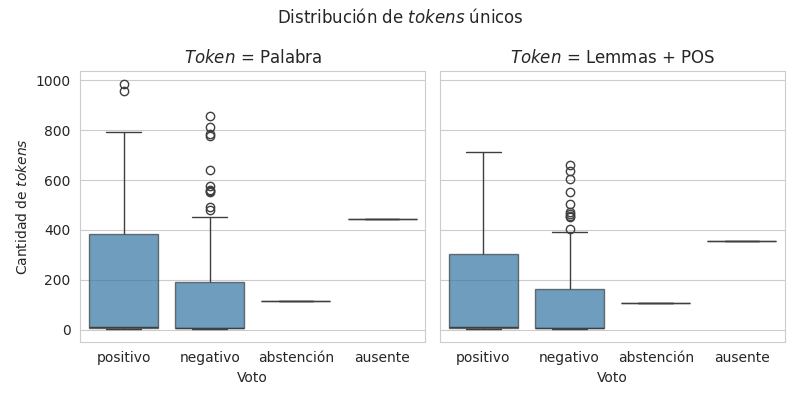
\includegraphics[scale=0.45]{../visualizations/distrib_tokes_vs_lemma_pos/distrib_tokens_vs_lemma_pos.png}
\caption{Distribuci\'on \textit{tokens} \'unicos aplicando distintos criterios de unicidad.}
\label{fig-distrib-unique-tokens}
\end{figure}